\section{Introduction} \label{sec:introduction}

Social networks, citation graphs, travel networks (roads, planes, trains, etc.), and product networks are just a few examples of existing graph datasets with anywhere from hudreds to billions of nodes and edges. Despite the obvious potential for learning from these massive, information-rich datasets, attempts at applying machine learning techniques to them have failed until recently. There has been extensive research in the area over the past decade and a recent paper published in 2017 by Kipf and Welling~\cite{Kipf2016} introduced a computationally efficent neural network model. Before diving into the details of their model, we discuss reason why traditional methods are insufficient for graph datasets. 

\subsection{Graph Datasets} \label{sec:network-datasets}
In a typical graph dataset, nodes have a set of features, called the \textit{feature vector} and a set of relationships with other nodes, called \textit{edges}. All graphs used in this paper are unweighted and are made to be undirected in preprocessing. While all nodes have a feature vector and edges, only some of them have a \textit{label}. Ultimately, our goal is to accurately label all unlabled nodes in the graph by learning from their relationships with labeled nodes. This is a semi-supervised learning problem since we are learning from both labeled and unlabeled data points. 


\begin{figure}
	\centering
	\begin{subfigure}{0.32\textwidth} % width of left subfigure 
		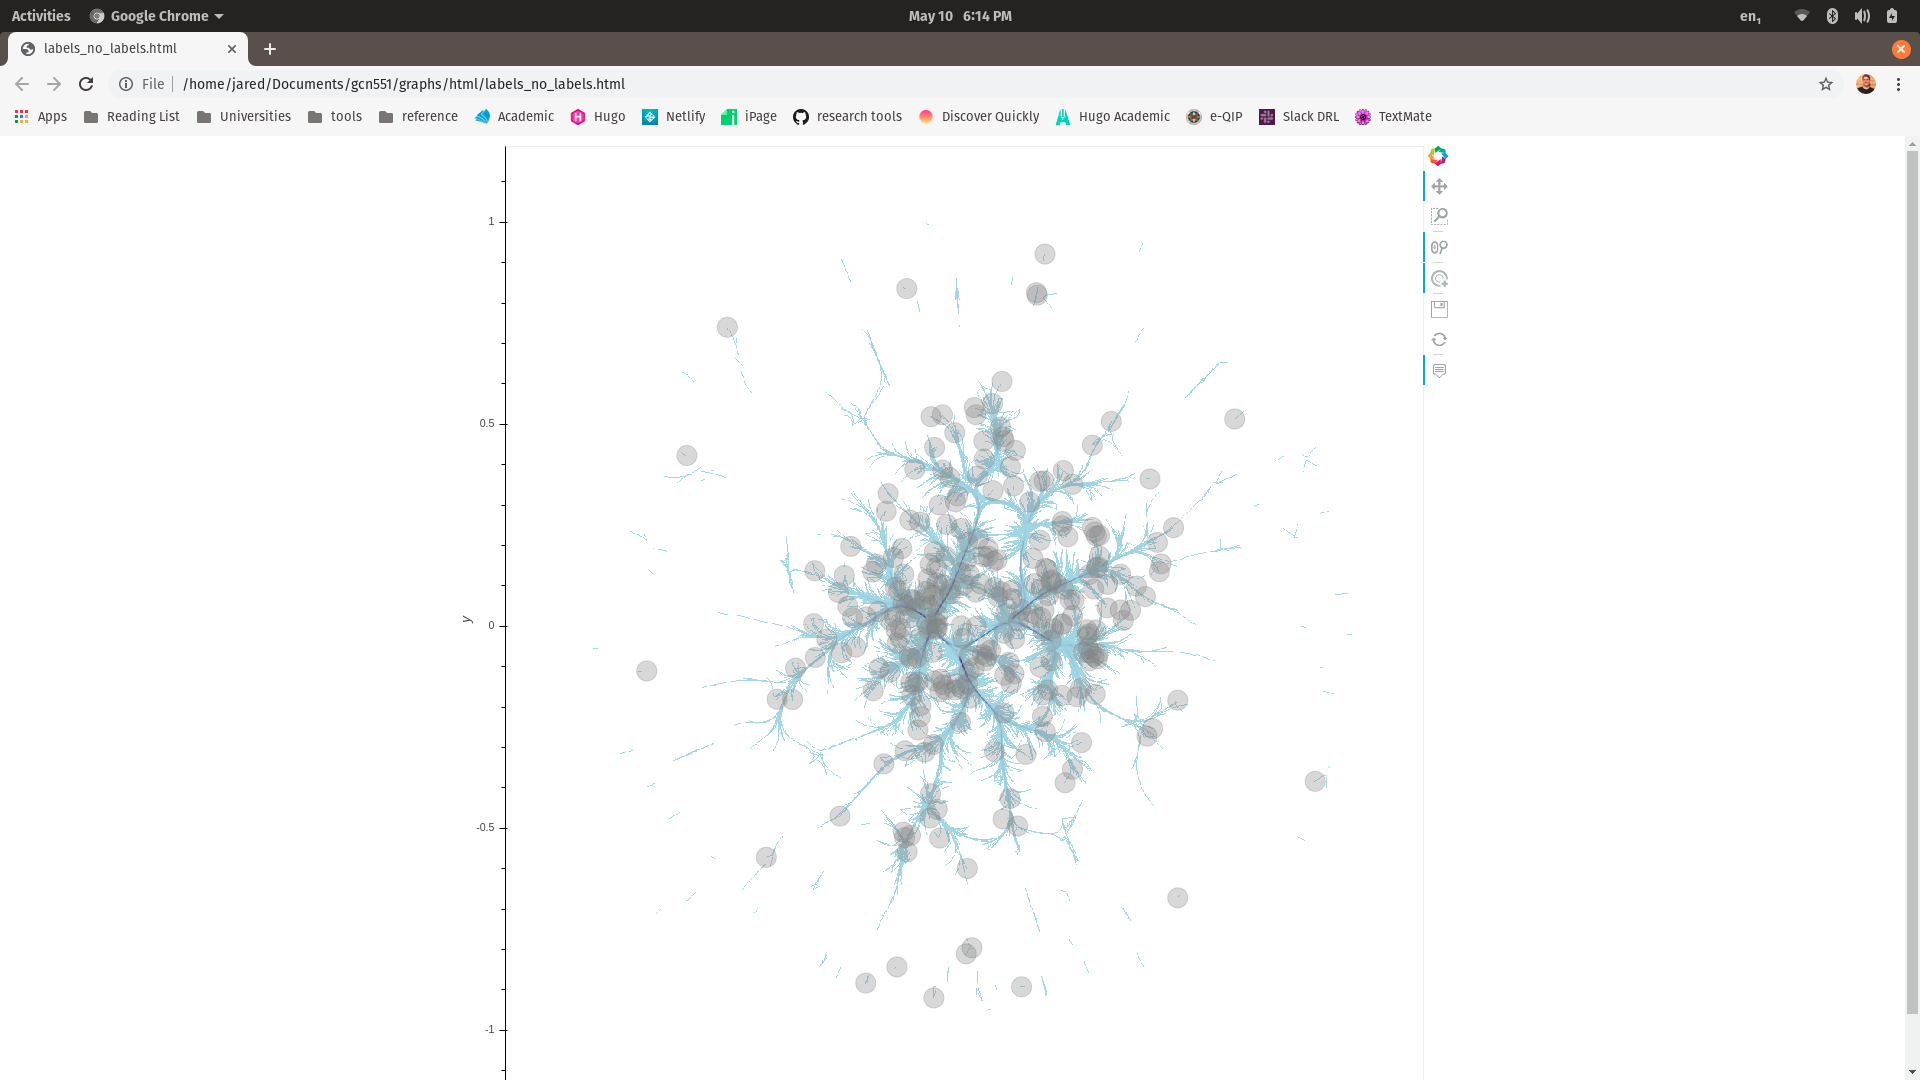
\includegraphics[width=\textwidth]{media/edges.png}
		\caption{Visualization of the edges of the network.} % subcaption
        \label{fig:dataset_edges}
	\end{subfigure}
	\vspace{1em} % here you can insert horizontal or vertical space
	\begin{subfigure}{0.32\textwidth} % width of left subfigure
		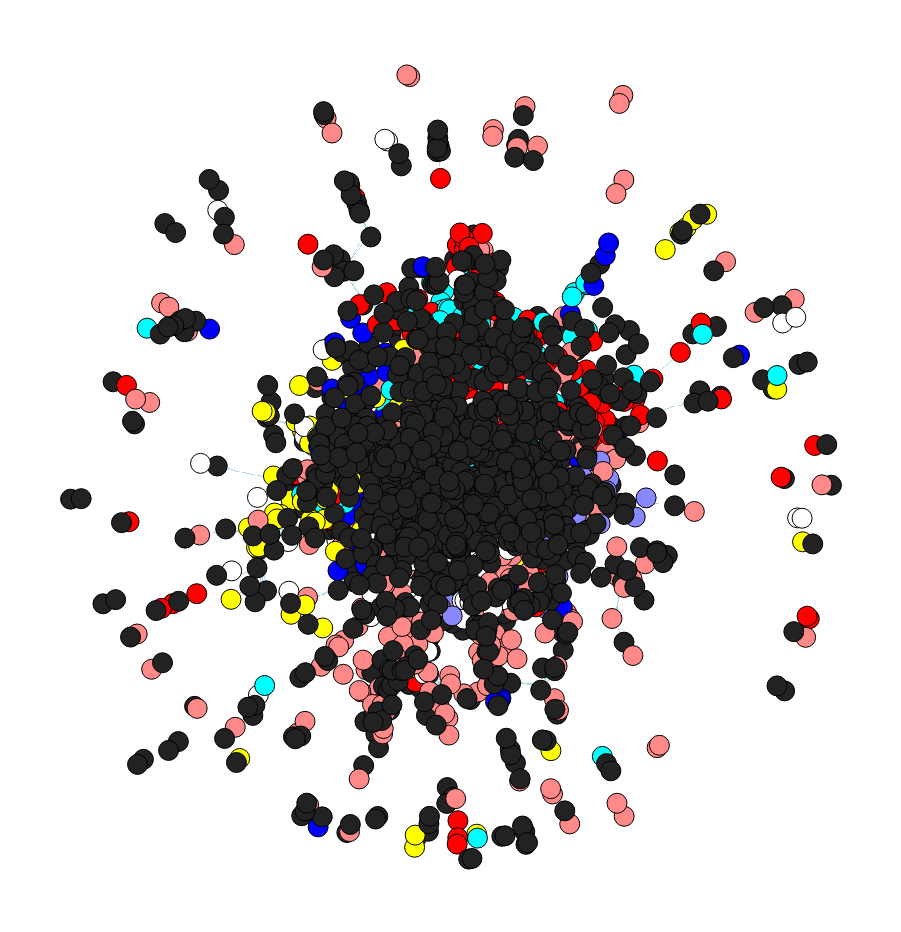
\includegraphics[width=\textwidth]{media/labels_only_train.png}
		\caption{Visualization of unlabled nodes in the network. It's clear that the vast majority of nodes are unlabled. This is the dataset our GCN will train on.} % subcaption
        \label{fig:dataset_all}
	\end{subfigure}
	\vspace{1em} % here you can insert horizontal or vertical space
    \begin{subfigure}{0.32\textwidth} % width of right subfigure
		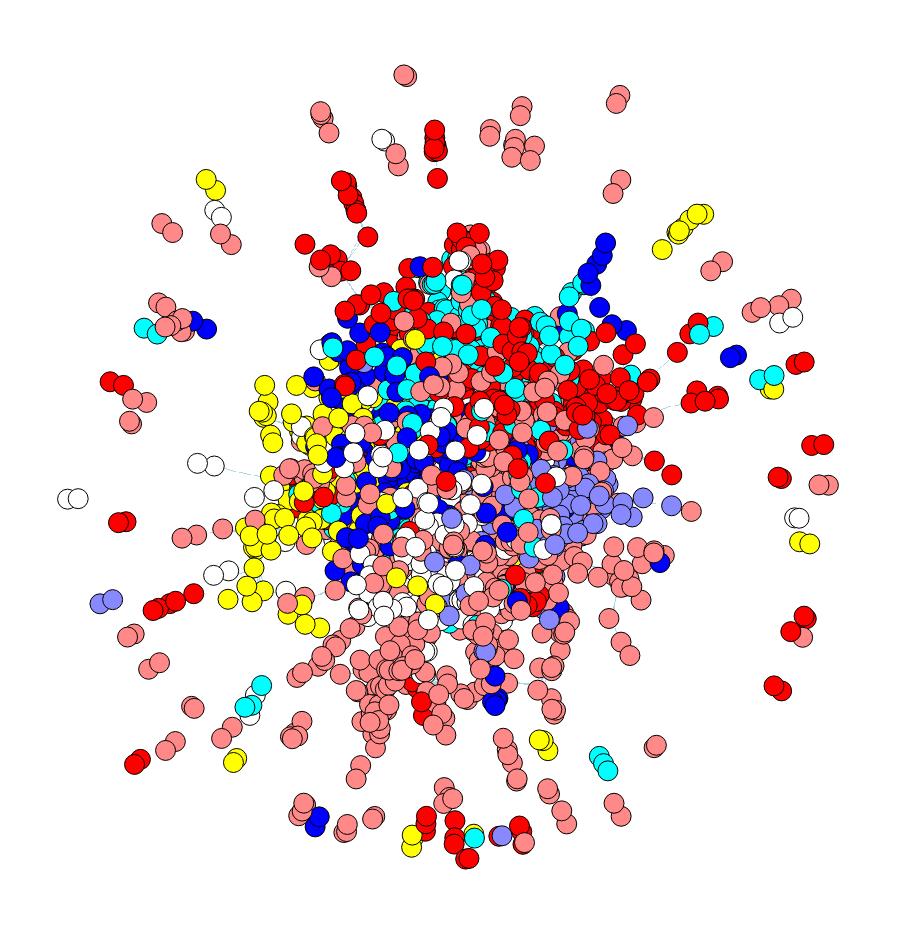
\includegraphics[width=\textwidth]{media/labels_all.png}
        \caption{Visualization of the dataset with all labels. For our experiments, our dataset actually has all labels. We remove all but twenty labels per class for training to simulate the sparsity with which a "real-world" dataset would be labeled. We use all labels at test-time to evaluate the accuracy of our model.} % subcaption
        \label{fig:dataset_train}
	\end{subfigure}
	\caption{Citeseer~\cite{} citation network visualization using the Fruchterman-Reingold force-directed algorithm. Even with a na\"ive drawing algorithm, clusers of equally-labeled nodes are visible. For this dataset, our goal is to recover \ref{fig:dataset_all} given \ref{fig:dataset_train}.} % caption for whole figure
\end{figure}


A good deep learning model for graphs should learn from both its nodes' feature vectors and its edges. This is based on the intuition that a node's neighboring feature vectors carry information about its own class. For example, in a social network, your close friends interests are likely to give some indication of your own (if all of your close friends like basketball, then you probably do too). The problem with traditional neural network methods is that they require regularly structured data. For example, Convolutional Neural Networks rely on information-rich matrices (e.g. pixels in an image). There is no obvious way to represent a graph and its features as a single regular structure. Adjacency matrices have regular structure, but are extremely sparse (Figure~\ref{fig:sparse}). In a Convolutional Neural Network, this would produce almost entirely zero-valued feature maps. 

\begin{figure}[h!]
	\centering
	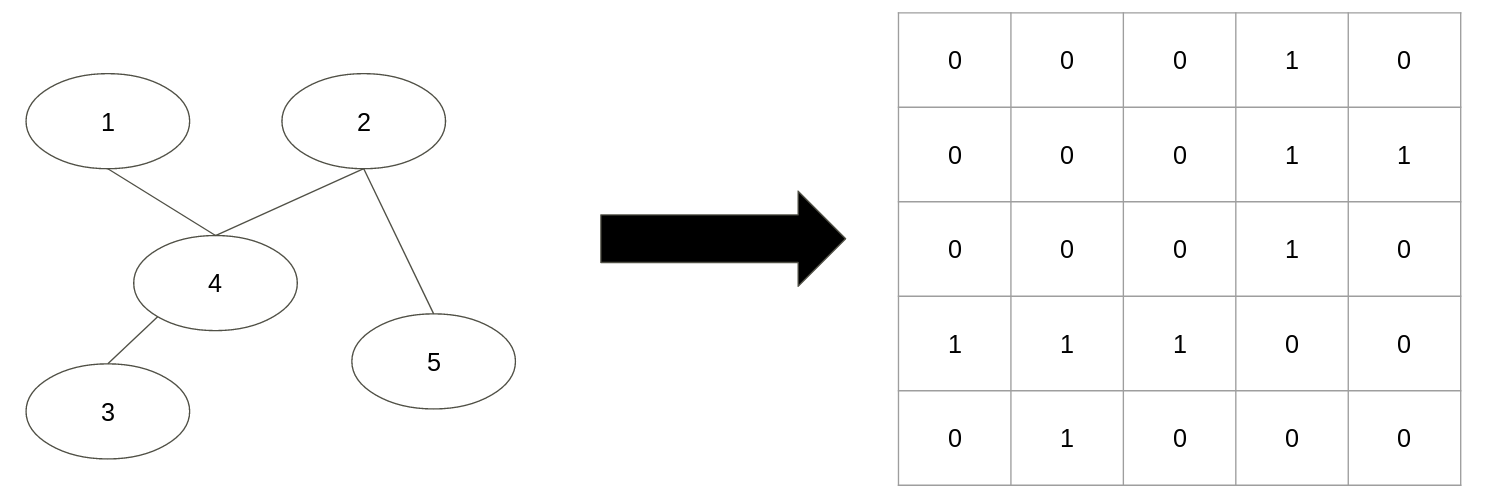
\includegraphics[width=1\linewidth]{media/sparse.png} 
	\caption{Adjacency matrices are extremely sparse. A Convolutional Neural Network, for example, would probably fail to produce decent results since small kernel sizes would be likely to create almost entirely zero-valued feature maps.}
	\label{fig:sparse}
\end{figure}
